\documentclass[10pt]{article}
\usepackage[utf8]{inputenc}
\usepackage[spanish]{babel}
\usepackage{fancyhdr}
\usepackage{graphicx}
\usepackage{boxedminipage}
\usepackage{array}
\usepackage{dsfont}
\usepackage{amsmath}
\usepackage{amsthm}
\usepackage{pgfgantt}
\usepackage{amssymb}
\usepackage{wasysym}
\usepackage{mathtools}
\usepackage[spanish,linesnumbered,ruled,vlined]{algorithm2e}
\usepackage{tikz}
\usetikzlibrary{arrows.meta,shapes,arrows,automata,babel}
\usepackage{float}
\usepackage{subcaption}
\usepackage{pgfgantt}
%\usepackage{stmaryrd}
\usepackage[pagebackref=true, breaklinks=true, letterpaper=true, colorlinks, bookmarks=false]{hyperref}
\hypersetup{
     colorlinks   = true,
     citecolor    = blue
}

\usepackage{xcolor} %to color text, in order to indentify changes
%made by your advisor. More info: https://www.sharelatex.com/learn/Using_colours_in_LaTeX

%color{OliveGreen} %new text
%color{Blue} %corrected text
%color{OrangeRed} %uncorrected text

%\topmargin  1 cm
\setlength{\textwidth}{15.5cm}
%\pdfpagewidth 9.5in
%\pdfpagewidth 5.5in
%\pdfpageheight 11in

\DeclareMathOperator*{\argmax}{arg\,max}
\DeclareMathOperator*{\argmin}{arg\,min}

\usepackage[left=3cm,top=2.5cm,bottom=2.5cm,right=3cm]{geometry}

\newtheorem{teorema}{Teorema}[section] %for theorem description

\renewcommand{\familydefault}{\rmdefault}

%compiles only desires pages, code extracted from http://tex.stackexchange.com/questions/96256/compiling-only-a-page-range-or-page-selection (04/20/2015)
\usepackage{lipsum,atbegshi,etoolbox}% http://ctan.org/pkg/{lipsum,atbegshi,etoolbox}
\makeatletter
\newcommand{\discardpages}[1]{% \discardpages{<csv list>}
  \xdef\discard@pages{#1}% Store pages to discard
  \AtBeginShipout{% At shipout, decide whether to discard page/not
    \renewcommand*{\do}[1]{% How to handle each page entry in csv list
      \ifnum\value{page}=##1\relax%
        \AtBeginShipoutDiscard% Discard page/not
        \gdef\do####1{}% Do nothing further
      \fi%
    }%
    \expandafter\docsvlist\expandafter{\discard@pages}% Process list of pages to discard
  }%
}
\newif\ifkeeppage
\newcommand{\keeppages}[1]{% \keeppages{<csv list>}
  \xdef\keep@pages{#1}% Store pages to keep
  \AtBeginShipout{% At shipout, decide whether to discard page/not
    \keeppagefalse%
    \renewcommand*{\do}[1]{% How to handle each page entry in csv list
      \ifnum\value{page}=##1\relax%
        \keeppagetrue% Page should be kept
        \gdef\do####1{}% Do nothing further
      \fi%
    }%
    \expandafter\docsvlist\expandafter{\keep@pages}% Process list of pages to keep
    \ifkeeppage\else\AtBeginShipoutDiscard\fi% Discard page/not
  }%
}

%\discardpages{24,25}% example of Discard these pages
%\keeppages{4}


%Header and Footer
\pagestyle{fancy}
\renewcommand{\headrulewidth}{0mm} %Para eliminar barra de header
\renewcommand{\footrulewidth}{0.4pt}
\newcommand{\tnhl}{\tabularnewline\hline}
\headheight 60pt
\lfoot{Proyecto de Tesis}
\rfoot{\thepage}
\cfoot{}
\rhead{}
\lhead{}
\chead{\setlength{\unitlength}{1mm}
\begin{picture}(0,0)
\put(-60,0){
\includegraphics[width=120mm]{logo-usm-di.png}}
\end{picture}}
\begin{document}



\section*{PROYECTO DE TESIS}
{\huge \Square} Doctorado en Ingeniería Informática

{\huge \CheckedBox} Magíster en Ciencias de la Ingeniería Informática


\begin{center}
\begin{tabular}{|%
    r @{ } %
    >{\bfseries\raggedright\hspace{1pt}} p{0.4\textwidth} |%
    >{\raggedright\hspace{0pt}}          p{0.5\textwidth} <{} |%
}\hline
   1.& Título del Proyecto de Tesis &
    A Content-Based Medical Image Retrieval for Pap Smear Images with Generative Adversarial Networks and Nearest Neighbor \tnhl

   2.& Nombre del Alumno            &
      Camilo Esteban Núñez Fernández         \tnhl

   3.& Número de Teléfono - Celular &
      (+56) 9 42131666         \tnhl

   4.& Correo electrónico           &
      camilo.nunezf@sansano.usm.cl    \tnhl

   5.& Fecha de Ingreso al Programa &
      2021 - 1  \tnhl

   6.& Pregrado \\ (Título o Grado Institución, Año) &
      Licenciado en Ciencias de la Ingeniería Informática,
      Universidad Técnica Federico Santa María, 2021\tnhl

   7.& Profesor Guía de Tesis       &    Mauricio Solar     \tnhl
   8.& Fecha Presentación Tema de Tesis &          \tnhl
   9.& Fecha Aprobación Tema de Tesis   &                       \tnhl
  10.& Fecha Tentativa de Término       & 30/07/2023      \tnhl
  11.& Comisión Interna de Graduación   &  %% \tabularnewline &&
                                          %YY \tabularnewline &&
                                          %ZZ
                                          \tnhl
\end{tabular}
\end{center}
%\normalsize

\newpage
\section*{Resumen}
\fbox{
\begin{minipage}[t][140mm][t]{0.95\textwidth}
\vspace{0.2cm}
%Contexto
El cáncer cervicouterino es el cuarto cáncer más común en mujeres en términos de incidencia y mortalidad en el mundo, y tercero en Chile. Debido a su actual prevalencia e impacto sobre la sociedad civil, es que se han realizado múltiples esfuerzos para su detección temprana por medio de tests. El test papanicolaou o pap smear test ha sido la metodología de detección temprana contra el cáncer cervicouterino más utilizado en el mundo.\\

%Problema
Sin embargo, al tratarse de un test de análisis de citología manual, sufre altos falsos positivos, además de existir un bajo ratio de análisis efectivo por parte de los citotecnólogos debido a la complejidad que lleva el análisis celular. Para sopesar esto, múltiples instituciones han implemento sistemas de recuperación de imágenes (CBIR) para la recomendación asistida en el proceso de análisis. No obstante, debido a los nuevos avances en la calidad de las imágenes y al gran volumen con el cual se generan, es que los CBIR deben aplicar mejores algoritmos para mejorar su funcionamiento.\\

%Propuesta y método usado para abordarlo
 El presente trabajo busca investigar, desarrollar e implementar un CBIR eficiente y robusto para imágenes médicas de papanicolaou. Para lograr ello, se utilizará una red neural generativa para la extracción de factores representativos de las imágenes, los cuales serán indexados comparados por medio de la técnica de grafos de vecinos más cercanos.\\

 %Validacion y hallazgo
Para validar y evaluar el CBIR propuesto se utilizaran los datasets ISBI Challenges 2014-2015, Herlev, SIPaKMeD y \textit{liquid-based cytology pap smear dataset}, y se compararan con modelos de extracción de factores representativos del estado del arte aplicados en distintos CBIR.\\

 %Implicaciones
Se espera que el CBIR propuesto pueda ser implementado en ambientes de producción clínicos como soporte en el análisis de citología para las muestras de papanicolaou en entidades nacionales e internacionales.

\vspace{10mm}

\textbf{Palabras Claves}: Cáncer cervicouterino, histopatologia, pap smear, content-based image retrieval, deep learning, generative adversarial networks, segmentación células cervicouterinas, clasificación células cervicouterinas, grafos vecinos más cercanos.
\end{minipage}}

\newpage
\section*{Abstract}
\fbox{
\begin{minipage}[t][120mm][t]{0.95\textwidth}
\vspace{0.2cm}
%Contexto
Cervical cancer is the fourth cancer type most common and deadliest among women in the world, being the thirds in Chile. Due to its current prevalence and impact on the society, multiple efforts have been made for their early detection through tests. The pap smear test has been the most commond screnning method used for the early detection against cervical cancer in the world.\\

%Problema
However, this test as it's a hand-operated method, suffers from high false positives cases, in addition to lowers effective rate of analysis by cytotechnologist due to the complexity involved in single-cell analysis. To solve this problem, multiple institutions have implemented content-based image retrieval (CBIR) systems for computer-aided in the analysis process. Nevertheless, due to new advances in the image quality and the large volume of date that generate this, CBIRs must apply better algorithms to improve the performance.\\

%Propuesta y método usado para abordarlo
This thesis proposed it's focused on investigate, develop and implement an efficient and robust CBIR for pap smear images. To achieve this, a novel generative neural network is proposed for the feature extraction of images, which will be indexed a retrieval by a graph-based nearest neighbor algorithm.\\

 %Validacion y hallazgo
The proposed CBIR will be evaluated and validated over the datasets ISBI Challenges 2014-2015, Herlev, SIPaKMeD and liquid-based cytology pap smear dataset, and will be compared with multiples features extraction methods availables in the current state of the arts.\\

 %Implicaciones
 The CBIR results are expected to assist medical specialists in the pap smear test analysis.

\vspace{10mm}

\textbf{Keywords}: Cervical cancer, cytopathology, pap smear, content-based image retrieval, deep learning, generative adversarial networks, cervical cell segmentation, cervical cell classification, nearest neighbor graph. 
\end{minipage}
}


\newpage
\section[]{Formulación General de la Problemática y Propuesta Tesis}

\subsection{Antecedentes Generales del Problema}
El cáncer cervicouterino es el cuarto cáncer más común en mujeres en términos de incidencia y mortalidad~\cite{9789283204480}. Debido a esto, la World Health Organization (WHO) a fomentado de manera constante programas orientados a la prevención y detección por medio de prevalencia en la evacuación de contra el \textit{human papillomavirus} (HPV) y la aplicación de métodos de \textit{screening} en los sistemas de salud a lo largo del mundo~\cite{9789283204480}.

En Chile durante los años  2010 y 2016 se registraron 164.239 egresos por causas oncológicas en mujeres, de entre los cuales las principales tres causas más frecuentes son cáncer de mama (52.189), seguido del cáncer a la tiroides (20.488), y cáncer cervicouterino (16.946)~\cite{PNC20182028}. Frente a esto, como política de prevención, el Departamento de Manejo Integral del Cáncer del Minsal, determinó como examen de prevención temprana para el cáncer cervicouterino, la aplicación del examen Papanicolaou (\textit{pap smear}) para grupos objetivos de mujeres entre 25 - 64 años~\cite{PNC20182028}.
De este modo, y en base a las políticas de prevención tanto en Chile como en el mundo, es que el método de histopatología más utilizado es el \textit{pap smear} o \textit{liquid-based cytology method}, debido a su bajo costo y alta efectividad ~\cite{Saslow2012, Davey2006, PNC20182028}.\\

La aplicación tradicional del \textit{pap smear} test consiste en la recolección de células desde la terminal \textit{squamocolumnar} del cervix, las cuales son puestas en un portaobjetos (\textit{glass slides}) para microscopio y examinadas por un citotecnólogo~\cite{canjclin.23.3.174, PAPANICOLAOU1941193}. Sin embargo, el proceso de análisis (\textit{screening process}) por parte del especialista es la fase más costosa en tiempo y recursos al momentos de efectuar el test~\cite{9179730}; a modo de ejemplo, esta fase toma entre 5 a 10 minutos de analizar por muestra de acuerdo a la dificultad de análisis de las células, esto provoca que un citotecnólogo no pueda analizar más de 70 muestras por día ~\cite{Elsheikh2012}.\\

Por lo anterior, y considerando además el aumento exponencial en los volúmenes de datos y en la mejor/mayor calidad de las imágenes que generan los nuevos instrumentos, es que se torna necesario el uso de sistemas de herramientas computaciones para la asistencia profesional al citotecnólogo durante la fase de diagnostico y análisis celular. Estos sistemas son identificados en la literatura como \textit{computer-aided diagnosis (CAD)}~\cite{DOI2007198}.

\subsection{Definición del Problema}
Los sistemas \textit{computer-aided diagnosis} pueden encontrarse en múltiples soluciones profesionales, siendo las más características los \textit{image-based diagnosis systems}~\cite{Mller2004}. Sin embargo, estos sistemas al contar con masivos volumen de datos almacenados, no permiten a los citotecnólogo, o tecnólogos en general, optimizar el estudio de los casos clínicos importantes al momento de referenciar regiones importantes en las imágenes de muestras, lo cual mantiene los tiempos de diagnósticos~\cite{10.1007/978-3-642-11769-5_1}.
Para sopesar esta situación, es que se vuelve menester el uso de sistemas recomendadores de imágenes, o \textit{Content-Based Medical Image Retrieval (CMBIR)} durante el proceso de análisis de las células~\cite{10.1117/12.769440}.\\

Los CMBIR, al ser una variante de los \textit{Content-Based Image Retrieval (CBIR)}, dependen de los \textit{features vectors} que puedan describir la imagen médica, los cuales pueden ser obtenidos por medios de \textit{handcraft-annotations} realizados por los profesionales, o por medio de técnicas supervisadas o no supervisadas de \textit{machine learning}~\cite{895972}.
Sin embargo, problemas como el \textit{overlapping} de células~\cite{Zhao2022}, la semántica general de la imágen~\cite{9046839}, la indexación eficiente y la ausencia de \textit{feedback-based}~\cite{9606873}, suelen afectar el desempeño de los CMBIR; parte de estos problemas pueden ser tratados al construir \textit{features} con descriptores más óptimos y robustos respecto a las propiedades de las imágenes.

\subsection{Marco Teórico}

\subsubsection{Content-based image retrieval}
Según lo mencionado anteriormente, los \textit{CMBIR} son una variante de los \textit{CBIR}, contando con la única diferencia en el tipo de imágenes que se indexan y se retorna al usuario, las cuales en este caso particular se tratan de \textit{pap smear images}. A su vez, un \textit{CBIR} es una técnica de búsqueda de imágenes, en donde dada una \textit{query}, se retornan las imágenes más similares según una métrica definida. Las métricas que se utilizan miden esencialmente la similaridad entre propiedades \textit{(features)} de los elementos visuales que describen a la imagen, y que van desde el color, la forma, la distribución espacial de los elementos, o las regiones de interés \textit{(ROI)}~\cite{Datta2008}. La extracción de estos \textit{features} es determinante al momento de indexar las imágenes que utilizará el sistema recomendador.

El workflow de un \textit{CBIR} se muestra en la Figura \ref{fig:mt:1a}. La composición del wolflow se centra en dos secciones, una offline en la cual \textit{features} ya extraídos de las imágenes son almacenados e indexados por el motor de búsqueda; y una online donde la \textit{image query} realizada por el usuario es procesa  y sus \textit{features} extraídos, los cuales son comparados con respecto a los \textit{features} ya indexados por medio de un algoritmo de similaridad.

\begin{figure}
    \centering
    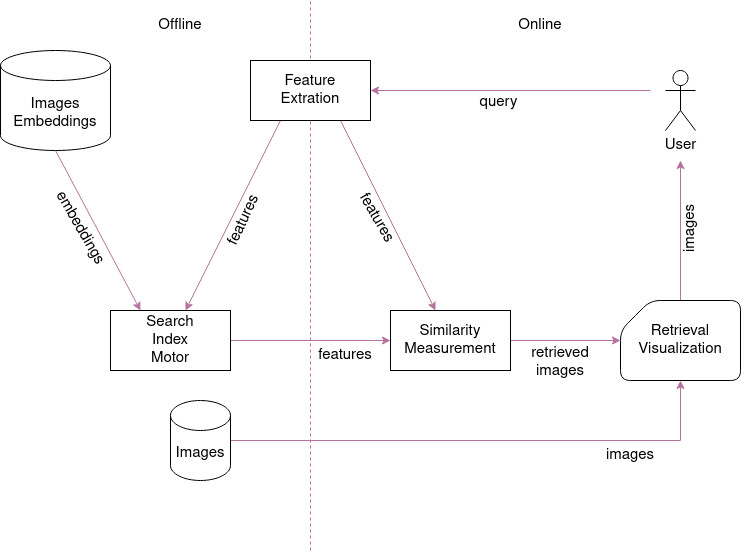
\includegraphics[width=0.6\textwidth]{img/cbir-flow.png}
    \caption{Worflow de funcionamiento de un CBIR. Se considera una parte offline, la cual corresponde a aquellos datos previamente calculados, como los \textit{features vectors} de las imagenes, y una parte online que considera la \textit{query image} ingresada por el usuario, la extracción de \textit{features} de esta imagen, el calculo de distancia con respecto a los vectores ya cálculos, y el retorno y visualización de las imágenes más cercanas. Imagen modifica desde \cite{Kumar2013}.}
    \label{fig:mt:1a}
\end{figure}

\subsubsection{Feature Extraction}
Un conjunto de tareas básicas que debe realizar un \textbf{computer-aided diagnosis} son la segmentación de la célula (incluyendo núcleo y citoplasma), la clasificación, y la extracción de \textit{features} ~\cite{Win2018}. Para resolver estas tareas, es posible aplicar múltiples técnicas de deep learning durante el procesamiento de las imágenes. Estas técnicas pueden ser supervisadas, semi-supervisadas o no supervisadas. Un detalle resumido de las principales técnicas utilizadas en el procesamiento de células de \textit{pap smear} se encuentra en la Figura \ref{fig:mt:2a}.
\begin{figure}
    \centering
    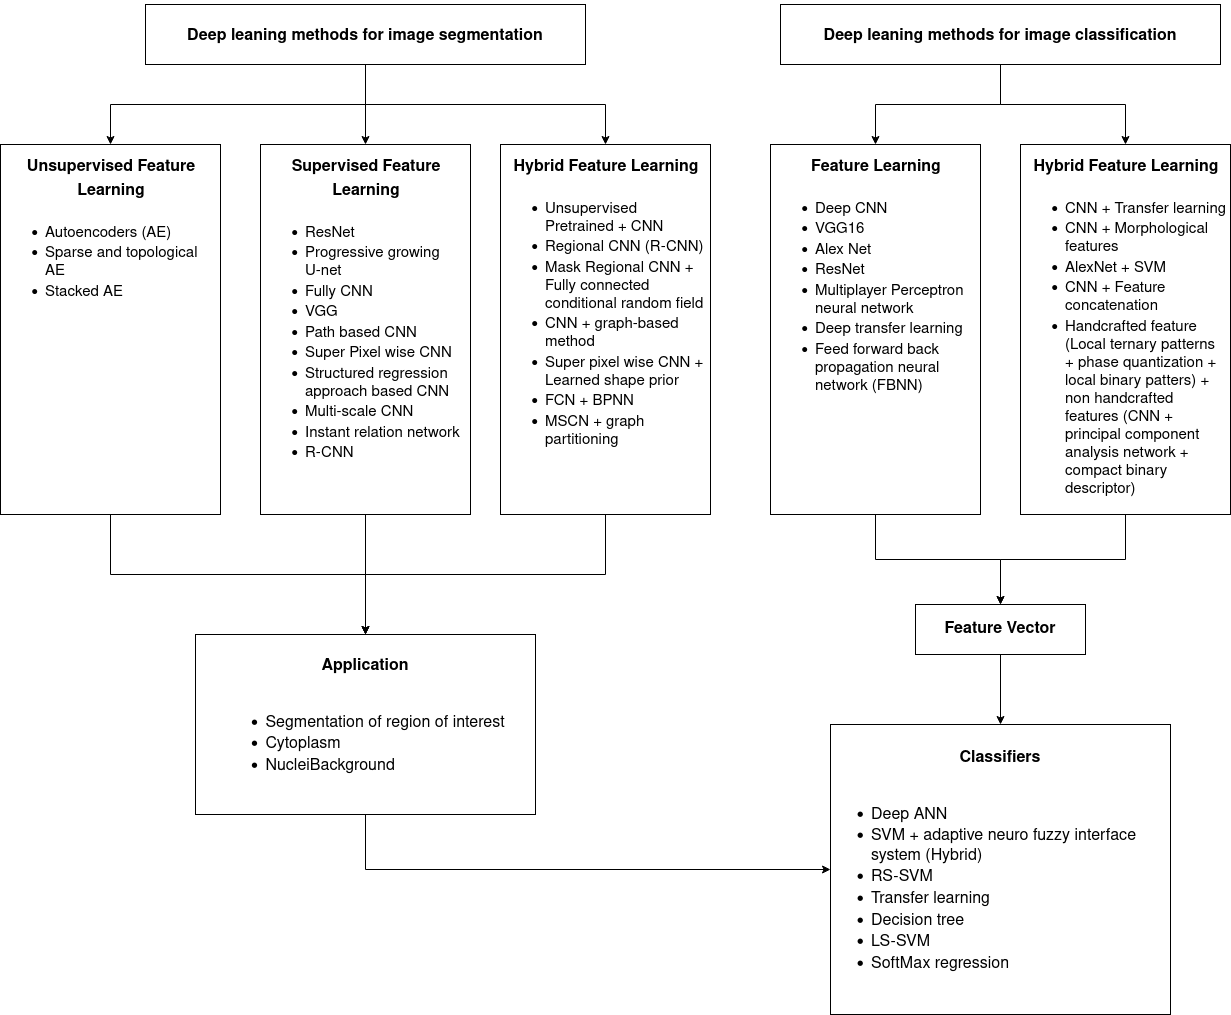
\includegraphics[width=0.9\textwidth]{img/dl-algo.png}
    \caption{Principales algoritmos de deep learning usados en el análisis de imágenes de \textit{pap smear}. Imagen modifica desde \cite{9046839}.}
    \label{fig:mt:2a}
\end{figure}
A partir de estas múltiples técnicas es que es posible crear distintos tipos de \textit{features vectors} tanto de la imagen original, como de las mascaras de segmentación (i.e. \textit{semantic mask} y \textit{boundary mask}), los cuales pueden ser usados a su vez como \textit{features vectors} para ser indexados. 

\subsection{Trabajos Relacionados}

\subsubsection{Content-based medical image retrieval para cáncer cervicouterino}
En materia de \textit{CMBIR}, es posible encontrar en la literatura como primer trabajo usando \textit{cervigram images} para el soporte en el diagnostico del cáncer Cervicouterino el realizado por \textit{Xue Z. et al.} en ~\cite{10.1117/12.769440}, donde se desarrolla un \textit{framework web} para la selección de múltiples \textit{ROI} de una \textit{query} dada, los cuales son procesados para su extracción de \textit{features} y comparados con valores pre-computados y almacenados en una base de datos. Los \textit{features} selecciones son el color, por medio de un histograma de intensidad de colores, la textura de la región obtenida por medio de la \textit{Discrete Wavelet Tranform}, y el tamaño de los \textit{ROI}. Estos tres \textit{features} son combinados y almacenados. Luego, al realizar una consulta, el usuario puede seleccionar la métrica de similaridad a usar, las cuales pueden ser \textit{Minkowski-form}, distancia de histogramas, divergencia de \textit{Jeffrey}, \textit{quadratic-form} y \textit{Earth mover's distance}. Finalmente, las métricas de evaluación usadas para el sistemas son \textit{precision} y \textit{accuracy}.\\

Un enfoque en el uso de \textit{CMBIR} para \textit{pap smear images} se puede encontrar en el trabajo de \textit{Mera M. et al.}~\cite{10.1007/s12553-015-0114-2}. En este trabajo, la extracción de \textit{features} se realizó por medio de \textit{Tamura textures}, \textit{Discrete Wavelet Tranform} y el cálculo de la matriz de co-ocurrencias. En esta oportunidad se utilizó el algoritmo de \textit{K-nearest neighbors} para retornar las $K$ imágenes más similares de acuerdo a la \textit{query} realizada por el usuario.\\

Respecto al uso de algoritmos de deep learning para la construcción de los \textit{features vectors}, es importante destacar los trabajos de \textit{Praveena H. et al.}~\cite{Praveena2022} para \textit{pap smear images} y de \textit{Ahmed A. et al.}~\cite{Ahmed2022} para \textit{cervigram images}.

En el caso del trabajo de \textit{Praveena H. et al.}, se realizó una propuesta híbrida de extracción de \textit{features}, por medio de una red \textit{ICNN} y los descriptores globales HOG~\cite{Nigam2018} y LBP~\cite{priya2018facial}; la recuperación de las imágenes se realizó por medio del calculo de similaridad usando la distancia \textit{chi-square}. Las métricas de evaluación utilizadas por los autores fueron \textit{accuracy}, \textit{precision}, \textit{specificity}, \textit{recall} y \textit{F-score}.

Respecto al trabajo de \textit{Ahmed A. et al.}, se utilizaron dos modelos para la extracción de \textit{features}, \textit{ResNet-18}~\cite{7839189} y \textit{SqueezeNet}~\cite{GOPALAKRISHNAN2017322}. Ambos modelos fueron pre-entrenados con el dataset \textit{ImageNet}~\cite{5206848} para aplicar \textit{transfer learning}. La métrica utilizada para la similaridad entre \textit{features vectors} fue distancia euclidiana. Para evaluar la performance del los modelos y del CMBIR, se utilizó las métricas de \textit{precision} y \textit{recall}.


\subsubsection{Feature Extraction para \textit{pap smear images}}
Los intereses en el desarrollo del presente proyecto de tesis se centrarán en dos técnicas \textit{state of the art} para la extracción de \textit{features} en \textit{pap smear images}: (I)~\textit{Generative Adversarial Networks} y (II)~\textit{Feature Distillation Network} para segmentación y clasificación.

\textit{Huang J. et al.} proponen la red \textit{Cell-GAN} en su trabajo~\cite{9513282}, para la segmentación de \textit{pap smear images}, por medio de un generador tipo encoder-decoder con doble entrada, una para la imagen y otra para un factor de guía, el cual indica la locación de los núcleos (\textit{guide factor}) de las células en una imagen completa, mientras la arquitectura usada en el discriminador corresponde a un modelo \textit{inception}~\cite{Vincent2008}. Dado que en este trabajo, el objetivo principal era generar la \textit{boundary mask} de una imagen, se utilizó el \textit{dice coefficiente} para evaluar la calidad de la segmentación.

Por otro lado, \textit{Ilyas T. et al.} proponen la red \textit{Tissue specific feature distillation network (TSFD-Net)}~\cite{Ilyas2022}, capaz de realizar las tareas de segmentación y clasificación simultáneamente. Esta red se compone de tres elementos principales: (I) un backbone primario para la extracción de \textit{features} utilizando la combinación de las arquitecturas \textit{Mobile-Net-v2}~\cite{10.48550/arxiv.1801.04381} y \textit{squeeze-excitation sub-network}~\cite{8578843}, (II) seguido de paths \textit{cross-scale weighted feature fusion (CWFF)} para la combinación de \textit{features}, reteniendo las propiedades espacial y locacional de la imagen; finalmente se considera un \textit{interlinked decoder (ID)} que corresponde a dos decoders interconectados, uno para la \textit{semantic mask} y otro para la \textit{boundary mask}. La arquitectura descrita se puede observar en la Figura \ref{fig:mt:3a}. Finalmente, los autores utilizaron la métrica \textit{Panoptic quality (QA)}~\cite{GRAHAM2019101563, 10.1007/978-3-030-23937-4_2} para evaluar el performance del proceso de segmentación, y las métricas de \textit{precision}, \textit{recall}, y  \textit{F-score} para el proceso de clasificación.
\begin{figure}
    \centering
    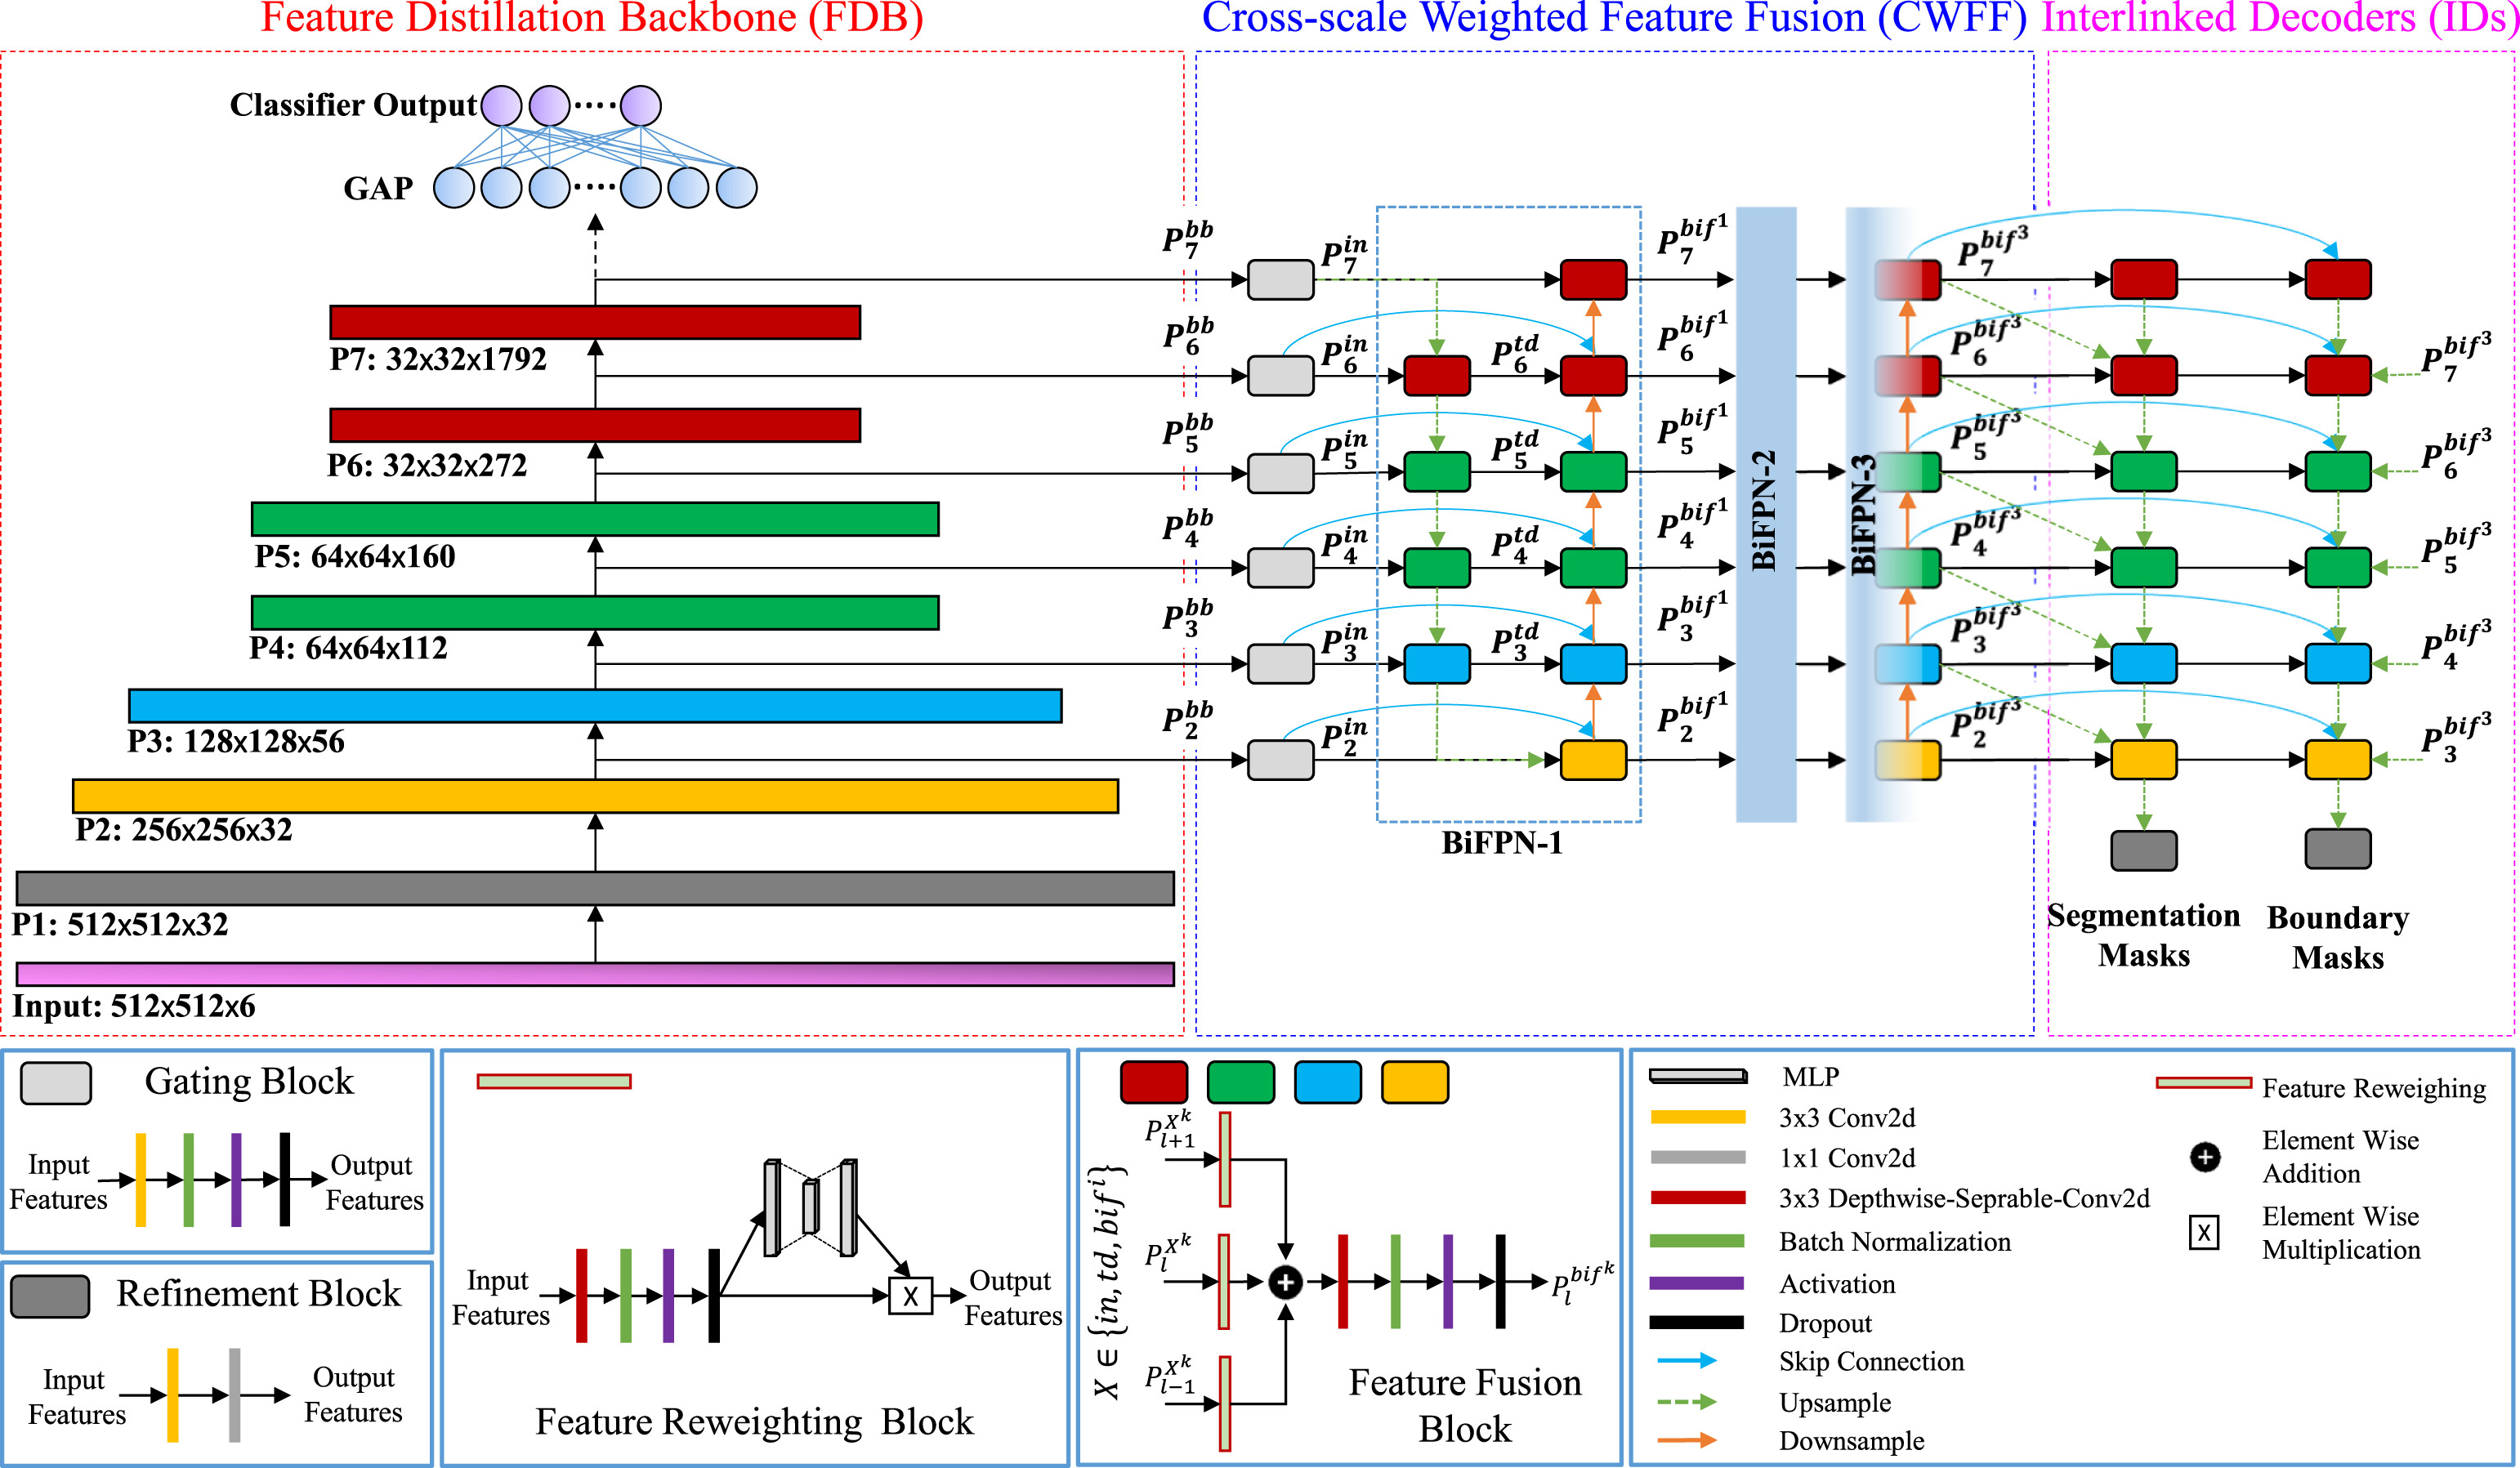
\includegraphics[width=0.8\textwidth]{img/1-s2.0-S0893608022000612-gr3_lrg.jpg}
    \caption{Arquitectura de la red \textit{TSFD-Net} propuesta por \textit{Talha Ilyas et al.}~\cite{Ilyas2022}.}
    \label{fig:mt:3a}
\end{figure}


\subsection{Propuesta de Tesis}
El desarrollo de esta tesis y su respectiva propuesta se centrará en la confección de un \textit{framework} para \textit{CMBIR} de imágenes \textit{pap smear}, con un enfoque \textit{computer-aided diagnosis} para las tareas de clasificación y segmentación. Este \textit{framework} tendrá la capacidad de recomendar tanto imágenes \textit{single-cell} como \textit{multi-cell} de acuerdo al tipo de búsqueda que deseé el usuario. Además de considerar a su vez la \textit{interlocation} de células similares en un tejido a analizar según el tipo de clasificación de la célula consultada (ver Figura \ref{fig:mt:4a}).\\

\begin{figure}
    \centering
    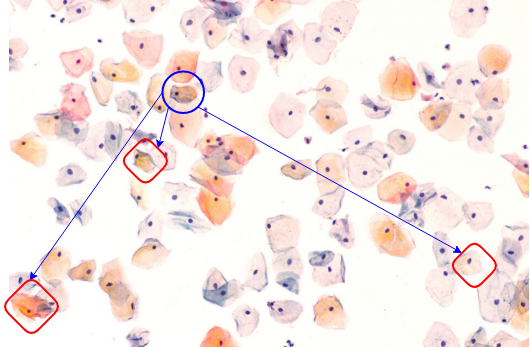
\includegraphics[width=0.5\textwidth]{img/multi-cell-1m.png}
    \caption{Consulta \textit{single cell} respecto a las demás células de una imagen \textit{pap smear}. El circulo en azul corresponde a la \textit{query} y los rombos en rojo a las células más similares a la \textit{query}.}
    \label{fig:mt:4a}
\end{figure}
Para desarrollar esta propuesta, se considerará la experimentación de múltiples combinaciones de \textit{features vectors} para indexar. Para ello se propone el análisis y estudio de un modelo generativo que incluye el entrenamiento de un generador de tres outputs: reconstrucción de una imagen \textit{pap smear}, su \textit{semantic mask} y \textit{boundary mask}. Además del entrenamiento de tres discriminadores, uno para output del generador. Esta arquitectura se muestre en la Figura \ref{fig:mt:5a}; a partir de este arquitectura, se busca estudiar la combinación de distintos tipos de \textit{features}, como los entregados por el backnocke del generador ($F_{backbone}$) o los entregados por los discriminadores ($F_{I}^{D},F_{SM}^{D},F_{BM}^{D}$).
\begin{figure}
    \centering
    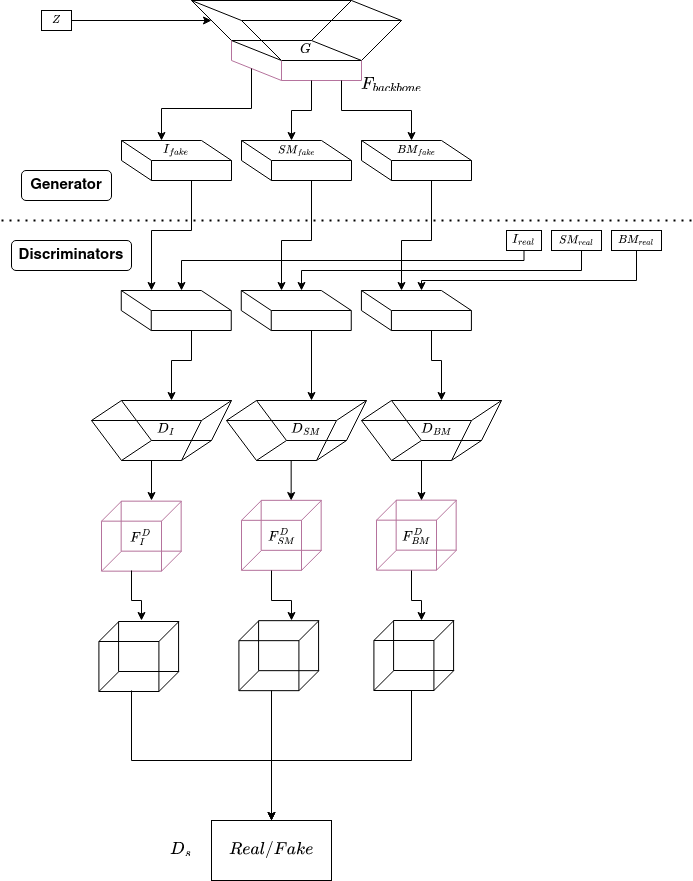
\includegraphics[width=0.7\textwidth]{img/arq-prop.png}
    \caption{Arquitectura propuesta para un modelo generativo con un único generador con múltiples \textit{outputs} y múltiples discriminadores para los \textit{outputs}.}
    \label{fig:mt:5a}
\end{figure}
Para el desarrollo del generador, se estudiara la factibilidad de modificación de la red \textit{TSFD-Net}~\cite{Ilyas2022}, particularmente el \textit{FDB}, para considerar ahora una reconstrucción total de la imagen original.\\

Para el entrenamiento de la red, se planea utilizar los datasets ISBI Challenges 2014-2015\cite{7005499}\cite{Lu2017},  Herlev~\cite{Marinakis2009}\cite{Dounias2006AutomatedIO}\cite{asljkhdjaskdj}\cite{86c7f5c1a9f84a7484731dd71671c563}, SIPaKMeD~\cite{8451588} y  liquid-based cytology Pap smear dataset~\cite{Hussain2020}, los cuales en total suman más de 6800 imágenes \textit{single-cell} y \textit{multi-cells} de \textit{pap smear}.\\

Finalmente, se estudiará el uso de un algoritmo \textit{graph-based} de Nearest Neighbor para el cálculo de similaridades entre los \textit{features vectors}. En particular se implementará el método \textit{HNSW}~\cite{Malkov2016EfficientAR, Boytsov2013EngineeringEA}, debido a sus excelentes resultados en el benchmark realizado por \textit{Aumüller M. et al.}~\cite{10.48550/arxiv.1807.05614}.

\newpage
\section[]{Hipótesis de Trabajo}


\fbox{
\begin{minipage}[t][30mm][t]{0.9\textwidth}
\vspace{0.2cm}
\begin{itemize}
    \item Es posible generar una combinación de \textit{features vectors} más robustos y de forma eficiente para un \textit{CMBIR} de imágenes \textit{pap smear} a partir de un red neural de clasificación y segmentación múltiple, entrenada de manera \textit{adversarial}.    
    \item El \textit{CMBIR} propuesto es capaz de mantener o superar el tiempo y la eficiencia en la recuperación de imágenes \textit{pap smear} respecto a otros \textit{CMBIR} del \textit{state of the art}.
\end{itemize}

\end{minipage}
}


\newpage
\section[]{Objetivos}%qué es lo que persigue la investigación
\subsection{Objetivos Generales}

\fbox{
\begin{minipage}[t][20mm][t]{0.9\textwidth}
\vspace{2mm}
El objetivo general de la presente propuesta es confeccionar e implementar un método eficiente de recuperación de imágenes médicas \textit{pap smear} por medio de similaridades en los descriptores que entregan los \textit{features vector} de las imágenes, extraídos por medio de redes neuronales.

\end{minipage}
}

\subsection{Objetivos Específicos} %metas que se deben lograr para llegar al objetivo general.
\fbox{
\begin{minipage}[t][115mm][t]{0.9\textwidth}
\vspace{2mm}
Los objetivos específicos de la presente propuesta son:
  \begin{enumerate}
    \item Identificar una arquitectura eficiente para generación de imágenes \textit{pap smear} y sus respectivas \textit{semantic mask} y \textit{boundary mask}.
    \item Identificar una arquitectura eficiente de discriminadores para la clasificación de imágenes \textit{pap smear} y sus respectivas segmentaciones.
    \item Implementar las arquitecturas descritas en el \textit{framework PyTorch} ~\cite{paszke2017automatic} en una unidad de GPU.
    \item Generar \textit{features vectors} a partir de las arquitecturas implementadas de imágenes seleccionadas de los datasets a utilizar.
    \item Identificar arquitecturas \textit{state of the art} para sus respectivas comparaciones respecto a las arquitecturas diseñas en la presente propuesta para la extracion de \textit{features}.
    \item Identificar un método eficiente para evitar el efecto \textit{curse of dimensionality} sobre los \textit{feaures vectors} generados.
    \item Implmentar el algoritmo \textit{HNSW} para la generación de índices para los \textit{feaures vectors} tanto de las arquitecturas propuestas como de las arquitecturas \textit{state of the art}.
    \item Comparar y analizar los resultados entregados por las implementaciones desarrolladas con respecto a otros métodos de \textit{CMBIR} para imágenes \textit{pap smear}.
    \item Elaborar un análisis cuantitativo y comparativo de los resultados obtenidos.
    \item Implementar la propuesta final en un \textit{framework web} para su disponibilidad académica.
  \end{enumerate}

\end{minipage}
}

\newpage
\section[]{Metodología y Plan de Trabajo}

\subsection{Plan de Trabajo}

\fbox{
\begin{minipage}[t][80mm][t]{0.9\textwidth}
\vspace{2mm}
El desarrollo del presente trabajo se estructura de acuerdo a la siguiente tabla de actividades:
\begin{table}[H]
\centering
\begin{tabular}{|l|c|}
\hline
\textbf{Actividad}         & \textbf{Tiempo {[}semana{]}} \\ \hline
Investigación y estudio del estado del arte & 2 \\
Implementación de los métodos estado del arte en \textit{PyTorch}& 2 \\
Identificación de los métodos y arquitecturas a utilizar & 2 \\
Implementación de los métodos identificados en \textit{PyTorch}& 2 \\
Identificación, recopilación y curación de datos & 2 \\
Experimentación y evaluación de las implementaciones & 2 \\
Validación y comparación respecto a otros métodos & 1 \\
Redacción y confección del documento de tesis & 3 \\
Correcciones    & 2 \\
Redacción y confección del documento a publicar & 2 \\ \hline
\textbf{Total}  & 20 \\ \hline
\end{tabular}
\end{table}
La proyección de desarrollo del trabajo en meses se proyecta de Marzo a Julio del semestre 2023-1.

\end{minipage}}


\newpage
\section[]{Resultados}
\subsection{Aportes y Resultados Esperados}

\fbox{
\begin{minipage}[t][122mm][t]{0.9\textwidth}
\vspace{2mm}
Los aportes y resultados realizados durante el presente trabajo se centraran en tres ejes: (I) reproducción del proyecto, (II) disponibilidad de datos procesados, (III) documentación \textit{long-term support}.

\subsubsection{Reproducción del Proyecto}
\begin{itemize}
    \item El desarrollo del proyecto deberá contar con una contenerización de dos etapas: un contenedor para el modulo de computo el cual contendrá tanto el \textit{enviroment} utilizado para ejecutar las arquitecturas y modelos, como su respectiva disponibilidad para la extracción de los \textit{features} en ambientes de producción, además de un contenedor para acceso \textit{web-based} por medio de una \textit{API REST}.
    \item La contenerización descrita deberá contar con una integración para aprovisionamiento en la nube para su despliegue en caso de un entorno de producción.
\end{itemize}

\subsubsection{Disponibilidad de Datos Procesados}
Tanto los \textit{embeddings} generados por el motor de indexación como los \textit{features vectors} obtenidos de los datos por medio de las redes serán dispuestos en un repositorio.

 \subsubsection{Documentación \textit{LTS}}
\begin{itemize}
    \item Se dispondrá de un repositorio con la documentación necesaria para replicar los experimentos realizados.
    \item Se documentará el proceso de puesta en marcha en producción en caso de uso en ambientes clínicos.
    \item Se versionará el proyecto de tesis realizado y se publicará un escrito en una conferencia o revista científica.
\end{itemize}

\end{minipage}
}

\subsection{Formas de Validación}

\fbox{
\begin{minipage}[t][63mm][t]{0.9\textwidth}
\vspace{2mm}
La validación de la presente propuesta considerará:
\begin{itemize}
    \item \textbf{Validación del CMBIR}: Al igual que en los trabajos de \textit{Ahmed A. et al.}~\cite{Ahmed2022} y \textit{Praveena H. et al.}~\cite{Praveena2022}, se considerarán las métricas de \textit{precision} y \textit{recall} para evaluar las imágenes retornas por el sistemas recomendador en los distintos casos propuestos.
    \item \textbf{Validación de imágenes generadas}: Se considerará el uso del \textit{dice coefficient} para la evaluación de las mascaras generadas, similar a lo expuesto en el trabajo de \textit{Huang J. et al.}~\cite{9513282}, y además el \textit{inception score (IS)}~\cite{NIPS2016_8a3363ab} y el Fréchet inception distance (FID)~\cite{10.48550/arxiv.1706.08500} para las imágenes generadas a partir de la reconstrucción, similar a lo expuesto en el trabajo de \textit{Zhao C. et al.}~\cite{Zhao2022}.
    \item \textbf{Validación clínica}: Se tomará en consideración la evaluación del sistema recomendador en producción por medio de un grupo clínico de especialistas por definir.
\end{itemize}
\end{minipage}
}

\newpage
\section[]{Recursos}
\subsection{Recursos Disponibles}
%Señale medios y recursos con que cuenta el Departamento de Informática de la UTFSM, para realizar el proyecto de tesis (libros, software, laboratorios, etc.). Su extensión no debe exceder el espacio disponible.

\fbox{
\begin{minipage}[t][50mm][t]{0.9\textwidth}
\vspace{2mm}
No Aplica
\end{minipage}
}

\subsection{Recursos Solicitados}
%Señale medios y recursos no disponibles en el Departamento de Informática de la UTFSM, necesarios para realizar el proyecto de tesis (libros, software, laboratorios, etc.). Su extensión no debe exceder el espacio disponible.

\fbox{
\begin{minipage}[t][50mm][t]{0.9\textwidth}
\vspace{2mm}
No Aplica
\end{minipage}
}

\newpage
% \bibliographystyle{ieeetr}
\bibliographystyle{alpha}
\bibliography{biblio}

\end{document}